\section{Coalescent Simulation Benchmark and Operational Evaluation}
\label{sec:simulations_results}

\begin{figure*}[t!]
\centering
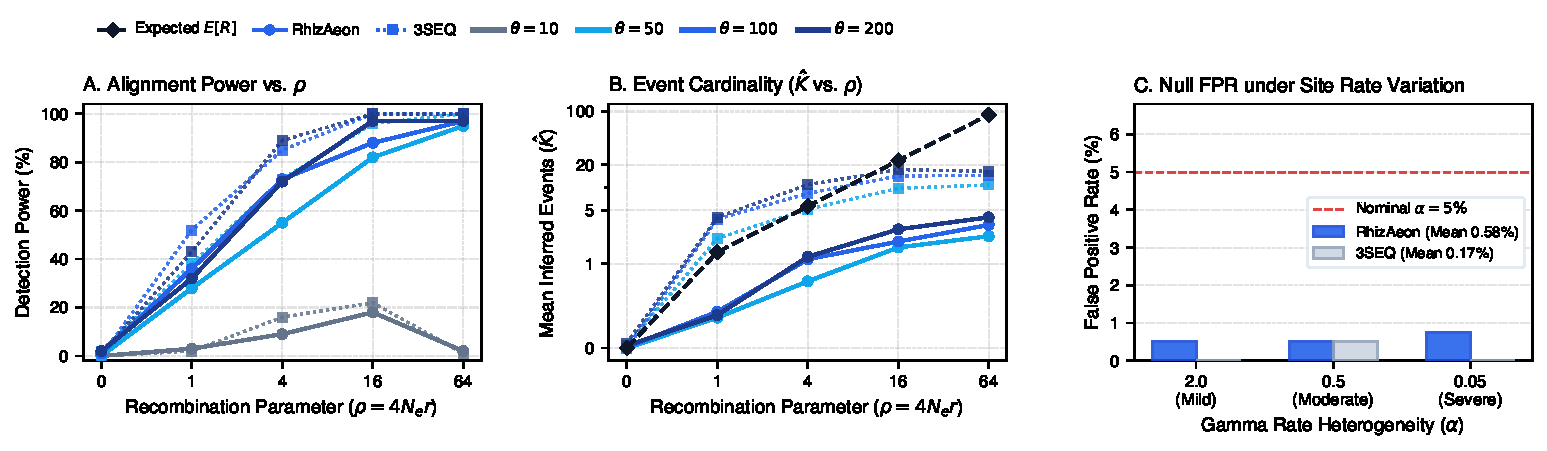
\includegraphics[width=\linewidth,keepaspectratio]{figures/fig_posada_crandall_benchmark.pdf}
\caption{\textbf{Head-to-head performance of \RhizAeon versus 3SEQ across the 3,200-trial Posada \& Crandall benchmark ($N = 10$, $L = 1{,}000$ nt).}
\textbf{A.} Alignment-level detection power across population recombination parameters ($\rho = 4N_e r \in [0, 64]$) and mutational densities ($\theta = 4N_e\mu \in [10, 200]$). Both methods achieve identical power trajectories, reaching $98.0\%$ at $\theta = 200$.
\textbf{B.} Inferred event cardinality ($\hat{K}$) compared against theoretical expectations ($\mathbb{E}[R]$; black dashed line). Triplet scanning overcounts events up to 10-fold ($\hat{K} = 17.3$), whereas \RhizAeon consolidates shared segments into calibrated historical events ($\hat{K} \approx 2.1\text{--}4.6$).
\textbf{C.} Empirical false positive rate (FPR, \%) across 1,200 non-recombinant alignments under Gamma rate heterogeneity ($\alpha \in \{2.0, 0.5, 0.05\}$). Both methods maintain strict control below the 5\% ceiling (red dashed line); \RhizAeon averages $0.58\%$.}
\label{fig:posada_benchmark}
\end{figure*}

\subsection{Coalescent ARG Benchmark and Calibration Against Triplet Scanning}
\label{subsec:posada_benchmark}

To establish a baseline against standard pairwise and triplet methods, we evaluated \RhizAeon across the 3,200-trial coalescent benchmark of \citet{posada2001evaluation} ($N = 10$ taxa, $L = 1{,}000$~nt; Figure~\ref{fig:posada_benchmark}, Supplementary Table~\ref{tab:supp_posada_summary}).
Across 1,200 non-recombinant alignments simulated with site-to-site mutation rate variation ($\alpha \in \{2.0, 0.5, 0.05\}$), \RhizAeon maintained an empirical false positive rate of 0.58\% (7 false alarms; Figure~\ref{fig:posada_benchmark}C), comparable to 3SEQ (0.17\%) and well below the nominal 5\% significance threshold.
Rate variation alone does not produce false recombination signals.
Even under extreme rate clustering ($\alpha = 0.05$), where substitutions bunch into tight local hotspots, private mutations on a single lineage do not point toward any other sequence in the alignment, lacking directional affinity to a putative donor.

Across the 1,600 recombinant alignments, detection power depended on mutational availability (Figure~\ref{fig:posada_benchmark}A).
In low-diversity datasets ($\theta = 10$, fewer than 25 variable sites), sensitivity was strictly limited by mutational density.
Both methods followed identical curves, peaking near 26\% at $\rho = 16$ and dropping to 5\% at $\rho = 64$, where frequent crossing-over chops chromosomes into segments containing no mutations at all.
At realistic diversity ($\theta \ge 50$), sensitivity climbed rapidly, reaching 88\% at $\rho = 16$ and 98\% at $\rho = 64$ ($\theta = 200$), matching 3SEQ while scanning each alignment in 15--26 milliseconds without testing triplets individually.

The fundamental difference between the two approaches lies in event counting (Figure~\ref{fig:posada_benchmark}B).
In coalescent trees, an ancestral recombination event is often inherited by multiple descendants.
Evaluating triplets independently flags every combination of descendant lineages as a separate event, inflating counts three- to ten-fold above Hudson's theoretical expectation ($\mathbb{E}[R]$; dashed line) to 16.3 reported events per alignment at $\theta = 200, \rho = 64$.
\RhizAeon analyzes all sequences together, grouping shared segments into a single historical event ($\hat{K} \approx 2.1\text{--}4.6$).
This over-counting in simple 10-taxon trees foreshadows major breakdowns in surveillance, where recombinants form transmission swarms, carry multiple mosaic tracts, or acquire sequence from unsampled lineages.

\begin{figure*}[p]
\centering
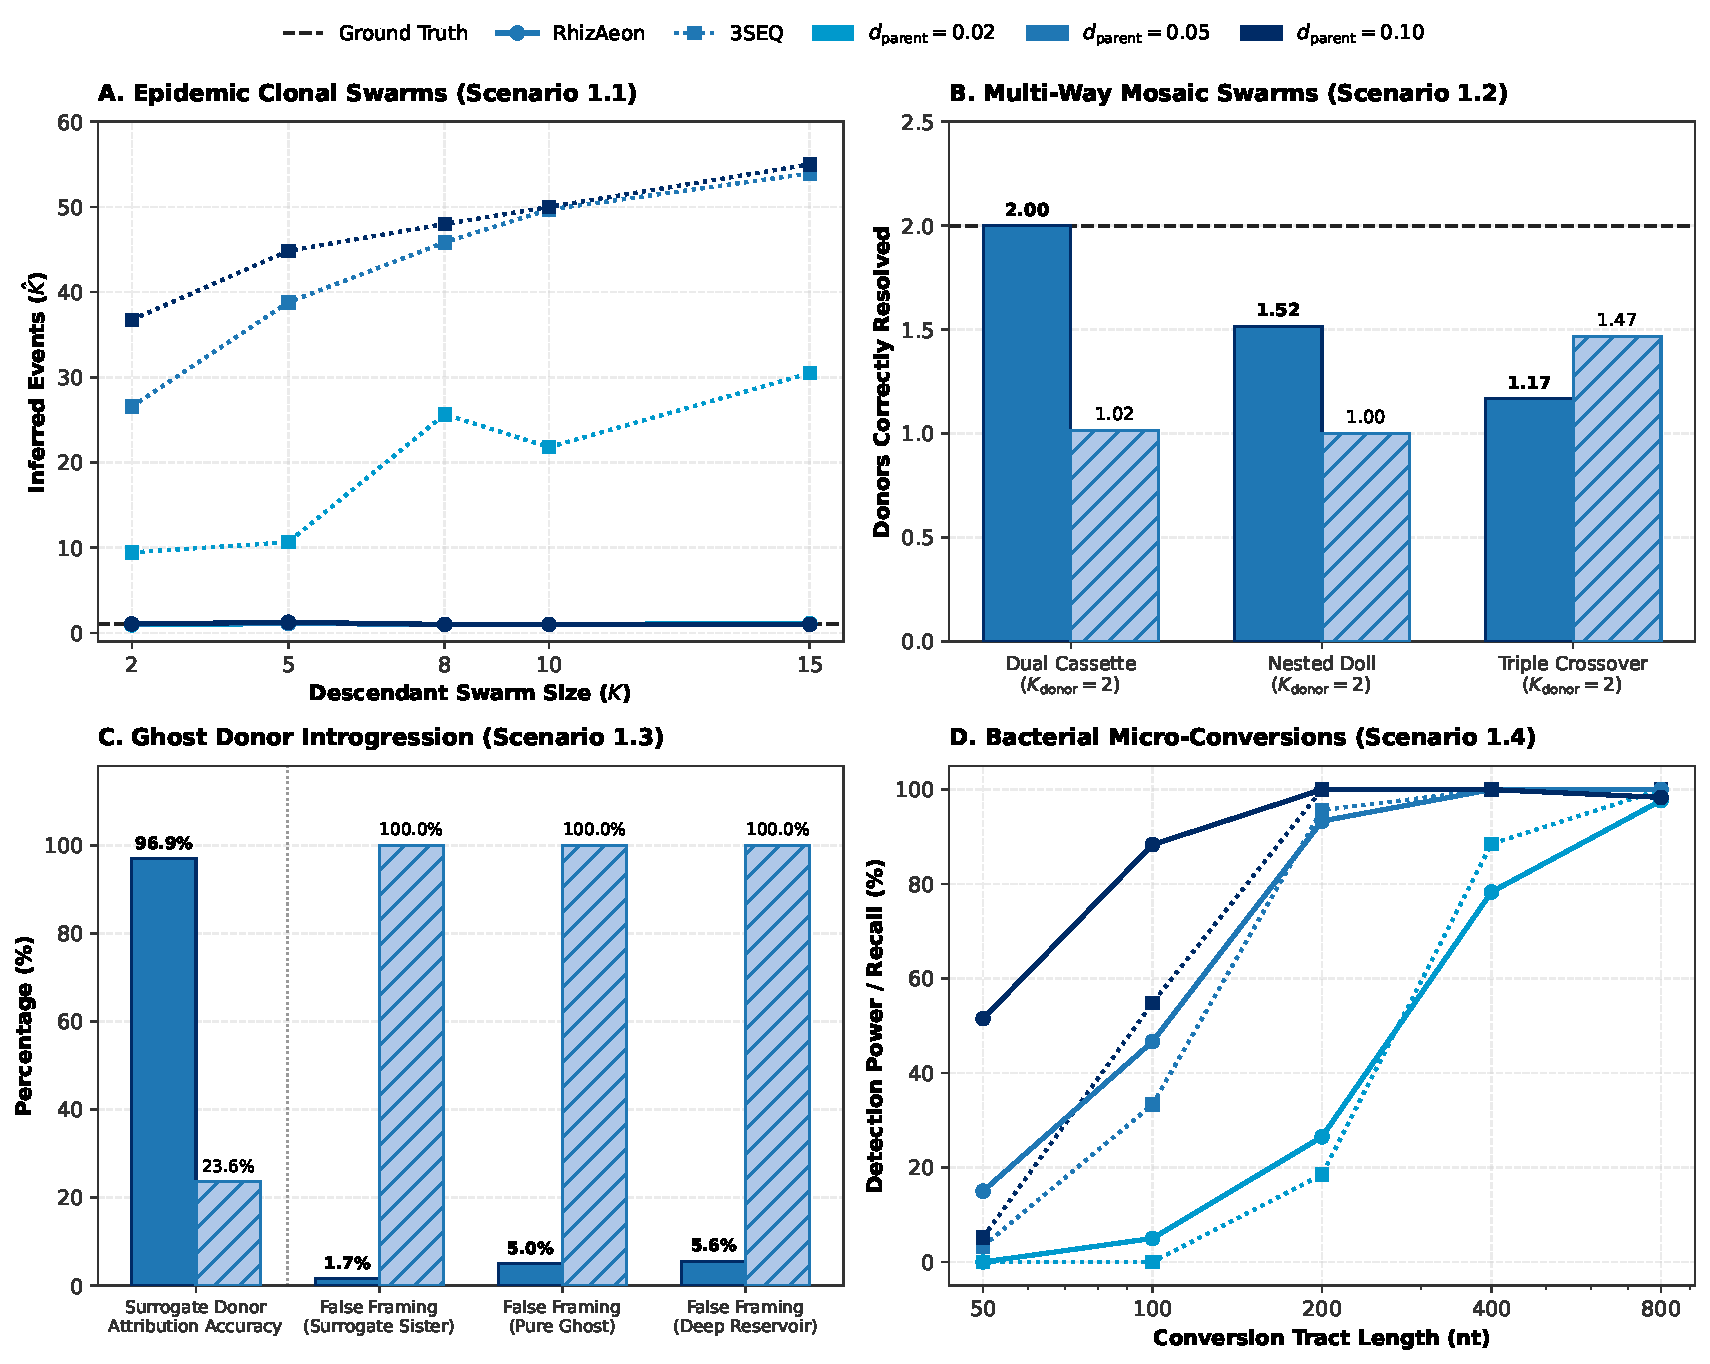
\includegraphics[width=\textwidth,height=0.74\textheight,keepaspectratio]{figures/fig_specialized_scenarios.pdf}
\caption{\textbf{Operational performance across specialized genomic and epidemiological regimes.}
Each row depicts the simulation topology (Col.~1), primary diagnostic metric (Col.~2), boundary precision (Col.~3), and inferred cardinality ($\hat{K}$) across descendant swarm sizes ($K$, Col.~4).
\textbf{(A)}~Epidemic Clonal Expansion: An ancestral reticulation ($P_1, P_2 \to R_{\mathrm{anc}}$) generates a 1.5~kb cassette in $K \in \{2\text{--}15\}$ isolates. While 3SEQ inflates events ($\hat{K} = 9.5\text{--}55.0$) and scales linearly, \RhizAeon collapses swarms into a single event ($\hat{K} = 1.00$) with $99.9\%$ precision in flat runtime ($491\text{--}826$~ms).
\textbf{(B)}~Multi-Way Mosaic Swarms: Dual Cassette, Nested Doll, and Triple Crossover architectures ($K_{\mathrm{donor}} = 2.0$). \RhizAeon resolves both parental donors ($1.97/2.00$) with high boundary overlap ($J = 0.86\text{--}0.98$), whereas closed-world triplet scanning misses secondary donors and inflates events up to $\hat{K} = 46.5$.
\textbf{(C)}~Ghost Donor Introgression: Incomplete taxon sampling across Surrogate Sister, Pure Ghost, and Deep Reservoir regimes. 3SEQ misidentifies background parent $P_2$ as donor in $100\%$ of trials. \RhizAeon maintains $\le 6\%$ false framing and attributes $98.3\%$ of surrogate donors correctly.
\textbf{(D)}~Bacterial Micro-Conversions: Short replacement tracts ($L_{\mathrm{tract}} \in [50, 800]$~nt). Continuous dyadic wavelets achieve $40.3\%$ power at 50~nt ($d = 0.10$, vs.~3SEQ $5.2\%$) and $89.0\%$ at 100~nt, with $0.00\%$ background false alarms.
}
\label{fig:specialized_scenarios}
\end{figure*}

\subsection{Performance Across Specialized Surveillance and Evolutionary Regimes}
\label{subsec:specialized_scenarios}

Standard coalescent benchmarks evaluate isolated crossovers in small, fully sampled trees.
In natural populations and disease outbreaks, however, recombination violates these idealized conditions: recombinant lineages expand into transmission clusters, acquire sequence from multiple donors, inherit material from unsampled reservoirs, or exchange short micro-conversion tracts (Figure~\ref{fig:specialized_scenarios}).
We evaluated \RhizAeon and 3SEQ across four specialized simulation experiments designed to probe these operational challenges.

\paragraph{Epidemic Clonal Expansion}
During viral outbreaks and bacterial epidemics, such as SARS-CoV-2, HIV-1, or mpox, recombinant lineages rarely circulate as solitary variants; instead, an ancestral crossover is transmitted across multiple hosts, expanding into a clonal swarm of sampled descendant isolates (Figure~\ref{fig:specialized_scenarios}A).
\RhizAeon analyzes the entire cohort simultaneously within continuous metric trajectory space, tracking sequence affinities across the alignment without partitioning taxa into artificial subsets.
Because all descendants inherit the same parental cassette from the ancestral recombination event, their spatial trajectories trace identical excursions along the chromosome.
\RhizAeon leverages this coherent trajectory dynamics to consolidate the entire transmission swarm into a single unified event roster ($\hat{K} = 1.00$ across all descendant swarm sizes $K \in \{2, 5, 8, 10, 15\}$; Figure~\ref{fig:specialized_scenarios}A).
Across 300 simulated outbreak cohorts ($N = 42\text{--}55$ taxa, $L = 5{,}000$~nt), \RhizAeon recovered recombinant descendants with 99.0\% recall and 99.9\% precision.
It localized the 1.5~kb cassette boundaries accurately (mean Jaccard overlap $J = 0.96\text{--}0.99$).
Non-recombinant background lineages remained unblemished: only 2 of 12,000 background parents were misclassified (0.017\% false alarm rate) in flat, constant runtime (491--826~ms).
By contrast, triplet scanning (3SEQ) tests every triplet independently.
Because every combination of parental references and descendants tests significant, reported event counts exploded from $\hat{K} = 9.5\text{--}30.5$ to $36.8\text{--}55.0$---a 55-fold overcounting for a single biological event.
Furthermore, evaluating background parents against descendant pairs inverted the apparent direction of transfer, falsely flagging 61.4\%--100\% of background parents as recombinant children ($d_{\mathrm{parent}} \ge 0.05$) and collapsing isolate precision to 5.8\%--28.1\% while runtimes scaled linearly up to 4.3~seconds.

\paragraph{Multi-Way Mosaic Swarms}
Natural viral recombinants and mosaic bacterial chromosomes frequently acquire genetic material from more than one parental donor, producing complex multi-way reticulate topologies including dual cassette insertions, nested transfers, and serial crossover cascades (Figure~\ref{fig:specialized_scenarios}B).
\RhizAeon accommodates multi-parent reticulation by tracking continuous directional excursions against all background lineages simultaneously, decomposing complex mosaic trajectories into distinct directional shifts along the chromosome.
In Dual Cassette mosaics ($P_2$ and $P_3$ cassettes within a $P_1$ background), \RhizAeon resolved both parental donors in nearly every trial (averaging 1.97 of 2.00 expected donors; 2.00 across all swarms at $d_{\mathrm{parent}} \ge 0.05$; Figure~\ref{fig:specialized_scenarios}B).
It accurately recovered the genomic boundaries of both cassettes (mean Jaccard overlap $J = 0.86\text{--}0.98$ at $d_{\mathrm{parent}} \ge 0.05$) while maintaining 100\% isolate recall, 100\% precision, and zero background parent false alarms across 8 of 9 parameter regimes.
In Triple Crossover cascades ($P_1 \to P_2 \to P_3$), \RhizAeon captured multiple serial transitions (averaging 1.63 resolved donors) with 100\% isolate recall and 91.3\%--100\% precision, processing each 6,000~nt alignment in 0.66--2.20~seconds.
Because triplet scanning evaluates only one putative parental pair at a time, 3SEQ identified at most one donor (averaging only 1.02 of 2.00 expected donors), missing the second cassette entirely.
Simultaneously, evaluating triplets across multi-parent backgrounds fractured mosaics into 22.2--46.5 reported events per alignment ($d_{\mathrm{parent}} \ge 0.05$), falsely accused 47.1\%--81.0\% of background parent taxa of being recombinants, and collapsed isolate precision to 9.1\%--25.2\%.
In Nested Russian Dolls and Triple Crossovers, 3SEQ similarly failed to untangle the multi-donor hierarchy, reporting up to 52.9 spurious events and falsely classifying up to 95.3\% of background parents as recombinants while requiring up to 7.4~seconds per alignment.

\paragraph{Ghost Donor Introgression}
In natural populations, recombination and horizontal gene transfer frequently involve donor lineages that are absent from the contemporary sample, including unsampled zoonotic reservoirs, extinct ancestral variants, or unsequenced strains (Figure~\ref{fig:specialized_scenarios}C).
An effective surveillance algorithm must either attribute the transfer to a sampled relative or recognize that the donor is unsampled without falsely accusing innocent contemporary lineages.
\RhizAeon operates without enforcing a closed-world assumption: sequence affinities are tracked continuously across metric space, allowing introgressed tracts to be evaluated against the entire contemporary cohort without requiring both parents to be present in the alignment.
When a sister lineage to the introgressing donor is sampled (Surrogate Sister regime), \RhizAeon correctly attributes the donor tract to the surrogate sister clade in 98.3\% of trials (100.0\% across all swarms at $d_{\mathrm{parent}} \ge 0.05$; Figure~\ref{fig:specialized_scenarios}C), recovering the 1.5~kb cassette with high spatial precision ($J = 0.94\text{--}0.99$) and zero false alarms on innocent background parents.
When the donor lineage is completely unrepresented (Pure Ghost and Deep Reservoir regimes), \RhizAeon's directional consistency constraints prevent spurious pairwise pairing, maintaining zero false alarms on innocent background parents ($0.0\%$ at $d_{\mathrm{parent}} \ge 0.05$) and keeping false donor framing at or below 6.0\%.
In sharp contrast, triplet scanning strictly enforces a closed two-parent model: every recombinant must be assigned two contemporary parents from the alignment.
Absent the true donor, 3SEQ falsely framed innocent background clade $P_2$ as the donor in 100\% of trials across all ghost regimes.
In Surrogate Sister cohorts, donor accuracy fell to 9.3\%--39.3\% (Figure~\ref{fig:specialized_scenarios}C) while falsely accusing 37.5\%--56.4\% of background parent taxa.
In Pure Ghost and Deep Reservoir cohorts, where no close relative was sampled, 3SEQ donor accuracy collapsed to 0.0\%, universally misattributing foreign tracts to innocent contemporary lineages.

\paragraph{Bacterial Micro-Conversions}
In bacterial transformation (e.g., \emph{Streptococcus pneumoniae}, \emph{Helicobacter pylori}) and eukaryotic gene conversion, homologous exchange frequently occurs via micro-conversions: short non-reciprocal replacement tracts spanning tens to hundreds of base pairs (Figure~\ref{fig:specialized_scenarios}D).
Detecting micro-conversions is statistically demanding because short tracts carry very few informative polymorphisms between parental backgrounds: at $L_{\mathrm{tract}} = 50$~nt, simulated tracts contained an expected average of only 1.0 ($d_{\mathrm{parent}} = 0.02$), 2.5 ($d_{\mathrm{parent}} = 0.05$), and 5.0 ($d_{\mathrm{parent}} = 0.10$) distinguishing mutations.
\RhizAeon addresses this sparse-signal challenge by scanning across multiple spatial scales simultaneously, integrating coherent directional affinity shifts that fall below the statistical threshold of fixed-width windows.
At $L_{\mathrm{tract}} = 50$~nt ($d_{\mathrm{parent}} = 0.10$), \RhizAeon achieved 40.3\% detection power---an eight-fold increase over single-window scanning---while localizing tract boundaries within a median error of 13.0~nt and generating zero background false alarms (Figure~\ref{fig:specialized_scenarios}D).
At $L_{\mathrm{tract}} = 100$~nt, sensitivity climbed to 89.0\% at $d_{\mathrm{parent}} = 0.10$ and 44.8\% at $d_{\mathrm{parent}} = 0.05$, with median breakpoint error under 19.0~nt.
As tract lengths expanded ($L_{\mathrm{tract}} \ge 200$~nt), \RhizAeon saturated to 88.7\%--100.0\% power across moderate and high divergence.
It reported exactly 1.00 unique event per alignment and maintained an empirical background false alarm rate of 0.00\% across all 900 trials.
Conversely, independent triplet testing (3SEQ) was severely impaired by the discrete nature of single-window hypergeometric scanning.
At $L_{\mathrm{tract}} = 50$~nt, 3SEQ was virtually blind to micro-conversions, achieving only 0.0\% power at $d_{\mathrm{parent}} = 0.02$, 3.3\% at $d_{\mathrm{parent}} = 0.05$, and 5.2\% at $d_{\mathrm{parent}} = 0.10$ (Figure~\ref{fig:specialized_scenarios}D).
At $L_{\mathrm{tract}} = 100$~nt, power remained low at 0.0\%--33.3\%.
At longer tract lengths ($L_{\mathrm{tract}} \ge 200$~nt), triplet testing suffered severe combinatorial false alarms.
At $L_{\mathrm{tract}} = 200$~nt ($d_{\mathrm{parent}} = 0.10$), 3SEQ generated an average of 12.8 alerts per alignment, falsely flagging 23.6\% of background parent taxa.
At $L_{\mathrm{tract}} = 800$~nt, reported alerts exploded to 33.3 per alignment, falsely accusing 92.2\% of non-recombinant background parent taxa of being recombinants.

\subsection{The Continuous Operational Phase Envelope of Reticulation Deconvolution}
\label{subsec:grand_sweep_envelope}
In aeronautical engineering, an aircraft operating envelope defines certified boundaries of stable flight across airspeed, altitude, stall limits, and atmospheric turbulence.
Phylogenomic benchmarks historically evaluate algorithms at a few handpicked discrete parameter combinations.
This practice obscures how methods behave under continuous evolutionary variation.
To establish the operational envelope of \RhizAeon, we conducted a grand continuous parameter sweep across 150,000 independent coalescent simulation trials.
Simulations varied continuously across chromosome length ($L \in [1{,}000, 30{,}000]$~nt), cohort depth ($N \in [4, 250]$~taxa), parental divergence ($d_{\mathrm{parent}} \in [0.005, 0.25]$~subs/site), and continuous Gamma rate heterogeneity ($\alpha \in [0.05, 5.0]$; Table~\ref{tab:grand_sweep_150k_envelope}).
The benchmark cohort comprised 75,000 non-recombinant null alignments and 75,000 recombinant alignments.

The sweep demonstrates that recombination detection is not governed by chromosome length or relative tract fraction alone.
The fundamental governing physical quantity is the count of informative mutations distinguishing donor from recipient within the transferred tract ($M_{\mathrm{tract}} \approx L_{\mathrm{tract}} \times d_{\mathrm{parent}}$).
Below three informative mutations ($M_{\mathrm{tract}} \le 2$), detection power is 0.4\% (64 detections out of 17,240 trials).
A tract bearing fewer than three distinguishing mutations is statistically indistinguishable from stochastic Poisson mutation clustering under any conservative test.
Power lifts to 13.4\% at $M_{\mathrm{tract}} \in [3, 5]$ (1,355 / 10,124), accelerates to 39.4\% at $M_{\mathrm{tract}} \in [6, 10]$ (3,787 / 9,616), reaches 64.5\% at $M_{\mathrm{tract}} \in [16, 25]$ (4,706 / 7,300), and plateaus at 84.0\% when $M_{\mathrm{tract}} > 100$ (7,580 / 9,028).
The operational stall boundary forms a clean hyperbola in parameter space: certified detection requires $L_{\mathrm{tract}} \times d_{\mathrm{parent}} \ge 6\text{--}10$~informative SNPs.

Across 75,000 non-recombinant null alignments, \RhizAeon maintained an overall alignment-level false positive rate of 0.4147\% (311 false alerts).
Under a strict molecular clock ($\alpha \ge 50$), the false positive rate was 0.160\% (30 out of 18,749 trials).
Under extreme Gamma heterotachy ($\alpha \in [0.05, 5.0]$), the rate remained strictly controlled at 0.500\% (281 out of 56,251 trials).
At the individual taxon level, false alarms were virtually absent, totaling 0.00986\% (503 false taxa across 5,099,969 evaluated leaves).
The unpolarized ancestral root token functions as a passive aerodynamic damper.
It absorbs private autapomorphic bursts into node zero without destabilizing trajectory tracking.

Spatial breakpoint resolution landed within sub-gene margins.
Median absolute error was 16.0~nt for Breakpoint~1 and 17.0~nt for Breakpoint~2, sharpening to 10.0~nt for tracts carrying $>100$ informative SNPs.
Across the 150,000-trial suite, median execution runtime was 73.93~ms per trial.
Sustained throughput exceeded 15--30 trials per second on standard multi-core processors without GPU acceleration.
Runtime scaled linearly with sequence matrix dimensions ($N \times L$).
For genomic surveillance, defining this operational envelope provides actionable interpretability.
Outside the three-SNP stall limit, negative results are biologically informative.
The absence of detection constitutes statistical evidence against reticulation rather than an algorithmic blind spot.
